\documentclass{article}
\usepackage[utf8]{inputenc}
\usepackage{hyperref}
\usepackage{breakurl}
\usepackage{textcomp}
\usepackage{graphicx}
\usepackage[catalan]{babel}
\title{Crossy Road \\
		\large Videojocs 2017/18 Q1}
\author{David Hernàndez Morales}

\begin{document}
\pagenumbering{gobble}
\maketitle
\newpage
\pagenumbering{arabic}
\section{Crossy Road}
El joc que s'intenta emular és Crossy Road \textsuperscript{\texttrademark}
publicat (i desenvolupat) el 20/11/2014 per \textit{Hipster Whale} \cite{webCrossy}
\cite{wikipediaCrossy}. A la figura \ref{logo} es pot veure el logo de Crossy Road 
amb l'emblemàtic pollastre que pretèn donar resposta a la pregunta 
\textit{Why did the chicken cross the road?} \cite{preguntaChicken} 

\begin{figure}[h!]
	\includegraphics[width=\linewidth]{Logo.png}
	\caption{Logo del crossy road}
	\label{logo}
\end{figure}

Com es pot veure a la taula \ref{dadesSortida}, el primer llençament va ser en
\textit{iOS}. Amb \textit{Android} un mes després i \textit{Windows Phone}
quasi un any més tard. També hi ha una versió per \textit{tvOS}.

\begin{table}[h!]
	\begin{center}		
		\label{dadesSortida}
		\begin{tabular}{l|l}
		\textbf{Plataforma} & \textbf{Data de sortida} \\
		\hline
		iOS & 20 Novembre, 2014 \\
		Android & 23 Decembre, 2014 \\
		Windows Phone & 1 Maig, 2015 \\
		tvOS & 30 Octubre, 2015		
		\end{tabular}
		\caption{Dates de sortida de Crossy Road.}
	\end{center}
\end{table}

L'objectiu del joc és avançar endavant evitant obstacles mòvils per la 
carretera i utilitzant plataformes. A l'imatge \ref{inGame}
es pot veure el tipus d'obstacles que s'han de superar.
Té moltes similituds amb el joc de
Frogger \textsuperscript{\texttrademark}, fins al punt que ha sigut
descrit com un ''endless Frogger'' per la premsa \cite{endlessFrogger1} 
\cite{endlessFrogger2}. La puntuació és el nombre de files superades i
el joc recorda el màxim al que has arribat. També hi ha monedes distribuïdes
per les diferents graelles. Quan el jugador triga molt en avançar, la càmera
el sobrepassa i una àguila l'atrapa. Per tant es marca des del principi molt
clarament l'objectiu. \newline

\begin{figure}
	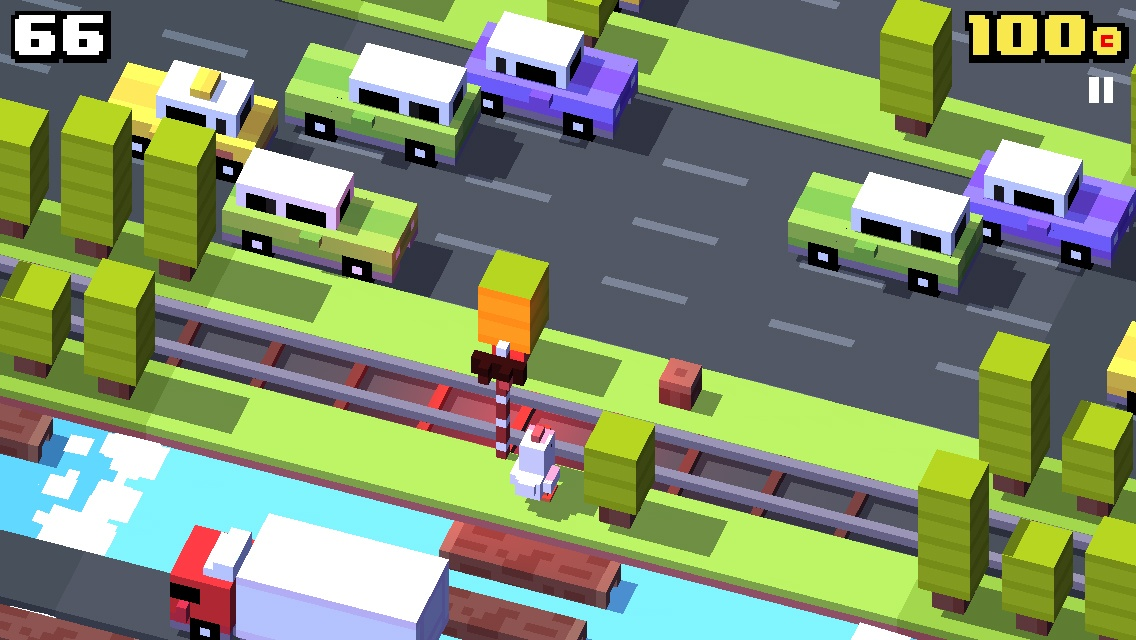
\includegraphics[width=\linewidth]{CrossyRoadGameplay.jpg}
	\caption{Imatge in-game de Crossy Road}
	\label{inGame}
\end{figure}

Cal afegir que el joc va treure dues versions addicionals. Una versió de 
Disney\textsuperscript{\textregistered} amb personatges com Mickey Mouse\textsuperscript{\texttrademark} i 
Donald Duck\textsuperscript{\texttrademark} i amb altres personatges
de franquícies de Disney com The lion king\textsuperscript{\texttrademark}
o Toy story\textsuperscript{\texttrademark} \cite{disneyCrossy}. També,
donat l'èxit de Star Wars\textsuperscript{\texttrademark}, es va treure
una versió de la franquícia ja que era massa gran per incloure-la en
la de Disney \cite{starWarsCrossy}. \newline

Inicialment estava planejat dedicar només 6 setmanes al Crossy Road, però vist el 
potencial del joc es va decidir deducar sis setmanes més \cite{delayedCrossy}. L'equip
de \textit{Hipster Whale} és un equip independent composat per Andy Sum i Mat Hall, els
fundadors, l'artista Ben Weatherall i la presidenta Clara Reeves \cite{HipsterPressKit}.
Algunes tecnologies utilitzades pel joc són \textit{Qubicle} \cite{qubicle} \cite{crossyPressKit} o \textit{Unity}.

Algunes referències a tenir en compte a més de la web oficial \cite{webCrossy} són la wiki feta per
fans \cite{crossyWiki} amb els diferents enemics i/o personatges, el trailer
de google play \cite{trailerCrossy} o aquest gameplay que mostra la corva de dificultat
del joc \cite{gameplayCrossy}

\section{Descripció del projecte}
Donat que el projecte intenta ser una còpia de \textit{Crossy Road}, els 
objectius bàsics són els mateixos: avançar tant com es pugui sense morir.
La puntuació és el nombre de files superades.

\section{Metodologia}
El desenvolupament d'aquest projecte ha sigut una mica especial, ja que 
al final he acabat presentant jo el projecte pel meu compte. Per tant,
donada la individualitat del projecte, no hi ha hagut reunions, ni fites, ni
diagrames de Gantt. Tampoc hi ha hagut sprints ni seguiment de
tasques mitjançant trello o slack perquè no tenia sentit sense
divisió de feina. \newline
Cal mencionar que en el joc 2D si que es va intentar utilitzar una metodologia 
similar a la cascada ja que es va dissenyar el diagrama UML de les classes
bàsiques i després implementarles iterativament. No obstant, en aquest cas
com que el projecte és de Unity, no ho he vist necessari. \newline
La dedicació de temps al projecte també ha sigut una mica erràtica ja que al principi confiava
en que el meu company fes la seva feina. Amb el temps em vaig adonar de que
no seria així i, per tant, no hi ha hagut un diagrama de Gantt, sinó més bé
un sprint constant per arribar al deadline. El que si que s'ha utilitzat és un control de versions, més concretament git
amb github. El github del projecte es pot trobar a \cite{githubProjecte}.

\section{Conclusions}
El projecte ha sigut molt interessant. El meu objectiu personal respecte a
aquesta assignatura era conèixer com és un videojoc per dins.
Puc dir que, després d'acabar el projecte i conjuntament amb les classes de
teoria tinc una noció bàsica del que suposa el desenvolupament de videojocs.
No obstant, he de dir que m'agradaria fer un videojoc des de zero només
amb C++ i OpenGL per realment comprendre tots els aspectes.
Si hagués tingut un company de treball adient, potser no hauriem utilitzat
Unity i hauriem començat desde zero que és el que m'hauria agradat a mi. 

\bibliography{Fonts}
\bibliographystyle{abbrv}
\end{document}